
\pdfminorversion=4 % for acroread
%\documentclass[aspectratio=169,t,xcolor={usenames,dvipsnames}]{beamer}
\documentclass[aspectratio=169,t,handout,xcolor={usenames,dvipsnames}]{beamer}
\usepackage{../beamerstyle}
\usepackage{dsfont}
\usepackage{bm}
\usepackage[english]{babel}
\usepackage[utf8]{inputenc}
\usepackage{graphicx}
\usepackage{algorithm}
\usepackage[ruled,vlined,algo2e,linesnumbered]{algorithm2e}
%\usepackage[boxed,vlined]{algorithm2e}
\usepackage{hyperref}
\usepackage{booktabs}
\usepackage{mathtools}

\usepackage{amsmath,amssymb}
\usepackage{listings}
\lstset{frame=lines,framesep=3pt,numbers=left,numberblanklines=false,basicstyle=\ttfamily\small}

\usepackage{subfig}
\usepackage{multicol}
%\usepackage{appendixnumberbeamer}
%
\usepackage{tcolorbox}

\usepackage{pgfplots}
\usepackage{tikz}
\usetikzlibrary{trees} 
\usetikzlibrary{shapes.geometric}
\usetikzlibrary{positioning,shapes,shadows,arrows,calc,mindmap}
\usetikzlibrary{positioning,fadings,through}
\usetikzlibrary{decorations.pathreplacing}
\usetikzlibrary{intersections}
\usetikzlibrary{positioning,fit,calc,shadows,backgrounds}
\pgfdeclarelayer{background}
\pgfdeclarelayer{foreground}
\pgfsetlayers{background,main,foreground}
\tikzstyle{activity}=[rectangle, draw=black, rounded corners, text centered, text width=8em]
\tikzstyle{data}=[rectangle, draw=black, text centered, text width=8em]
\tikzstyle{myarrow}=[->, thick, draw=black]

% Define the layers to draw the diagram
\pgfdeclarelayer{background}
\pgfdeclarelayer{foreground}
\pgfsetlayers{background,main,foreground}

%\usepackage{listings}
%\lstset{numbers=left,
%  showstringspaces=false,
%  frame={tb},
%  captionpos=b,
%  lineskip=0pt,
%  basicstyle=\ttfamily,
%%  extendedchars=true,
%  stepnumber=1,
%  numberstyle=\small,
%  xleftmargin=1em,
%  breaklines
%}

 
\definecolor{blue}{RGB}{0, 74, 153}

\usetheme{Boadilla}
%\useinnertheme{rectangles}
\usecolortheme{whale}
\setbeamercolor{alerted text}{fg=blue}
\useoutertheme{infolines}
\setbeamertemplate{navigation symbols}{\vspace{-5pt}} % to lower the logo
\setbeamercolor{date in head/foot}{bg=white} % blue
\setbeamercolor{date in head/foot}{fg=white}
\setbeamercolor{author  in head/foot}{bg=white} %blue
\setbeamercolor{title in head/foot}{bg=white} % blue
\setbeamercolor{title}{fg=white, bg=blue}
\setbeamercolor{block title}{fg=white,bg=blue}
\setbeamercolor{block body}{bg=blue!10}
\setbeamercolor{frametitle}{fg=white, bg=blue}
\setbeamercovered{invisible}

\makeatletter
\setbeamertemplate{footline}
{
  \leavevmode%
  \hbox{%
  \begin{beamercolorbox}[wd=.333333\paperwidth,ht=2.25ex,dp=1ex,center]{author in head/foot}%
%    \usebeamerfont{author in head/foot}\insertshortauthor
  \end{beamercolorbox}%
  \begin{beamercolorbox}[wd=.333333\paperwidth,ht=2.25ex,dp=1ex,center]{title in head/foot}%
    \usebeamerfont{title in head/foot}\insertshorttitle
  \end{beamercolorbox}%
  \begin{beamercolorbox}[wd=.333333\paperwidth,ht=2.25ex,dp=1ex,right]{date in head/foot}%
    \usebeamerfont{date in head/foot}\insertshortdate{}\hspace*{2em}
%    \insertframenumber\hspace*{2ex} 
  \end{beamercolorbox}}%
  \vskip0pt%
}
\makeatother

%\pgfdeclareimage[height=1.2cm]{automl}{images/logos/automl.png}
%\pgfdeclareimage[height=1.2cm]{freiburg}{images/logos/freiburg}

%\logo{\pgfuseimage{freiburg}}

\renewcommand{\comment}[1]{
	\noindent
	%\vspace{0.25cm}
	{\color{red}{\textbf{TODO:} #1}}
	%\vspace{0.25cm}
}
\newcommand{\notefh}[1]{\textcolor{red}{\textbf{FH:} #1}}
\renewcommand{\comment}[1]{}
\newcommand{\hide}[1]{}
\newcommand{\cemph}[2]{\emph{\textcolor{#1}{#2}}}

\newcommand{\lit}[1]{{\footnotesize\color{black!60}[#1]}}

\newcommand{\litw}[1]{{\footnotesize\color{blue!20}[#1]}}


\newcommand{\myframe}[2]{\begin{frame}[c]{#1}#2\end{frame}}
\newcommand{\myframetop}[2]{\begin{frame}{#1}#2\end{frame}}
\newcommand{\myit}[1]{\begin{itemize}#1\end{itemize}}
\newcommand{\myblock}[2]{\begin{block}{#1}#2\end{block}}


\newcommand{\votepurple}[1]{\textcolor{Purple}{$\bigstar$}}
\newcommand{\voteyellow}[1]{\textcolor{Goldenrod}{$\bigstar$}}
\newcommand{\voteblue}[1]{\textcolor{RoyalBlue}{$\bigstar$}}
\newcommand{\votepink}[1]{\textcolor{Pink}{$\bigstar$}}

\newcommand{\diff}{\mathop{}\!\mathrm{d}}
\newcommand{\refstyle}[1]{{\small{\textcolor{gray}{#1}}}}
\newcommand{\hands}[0]{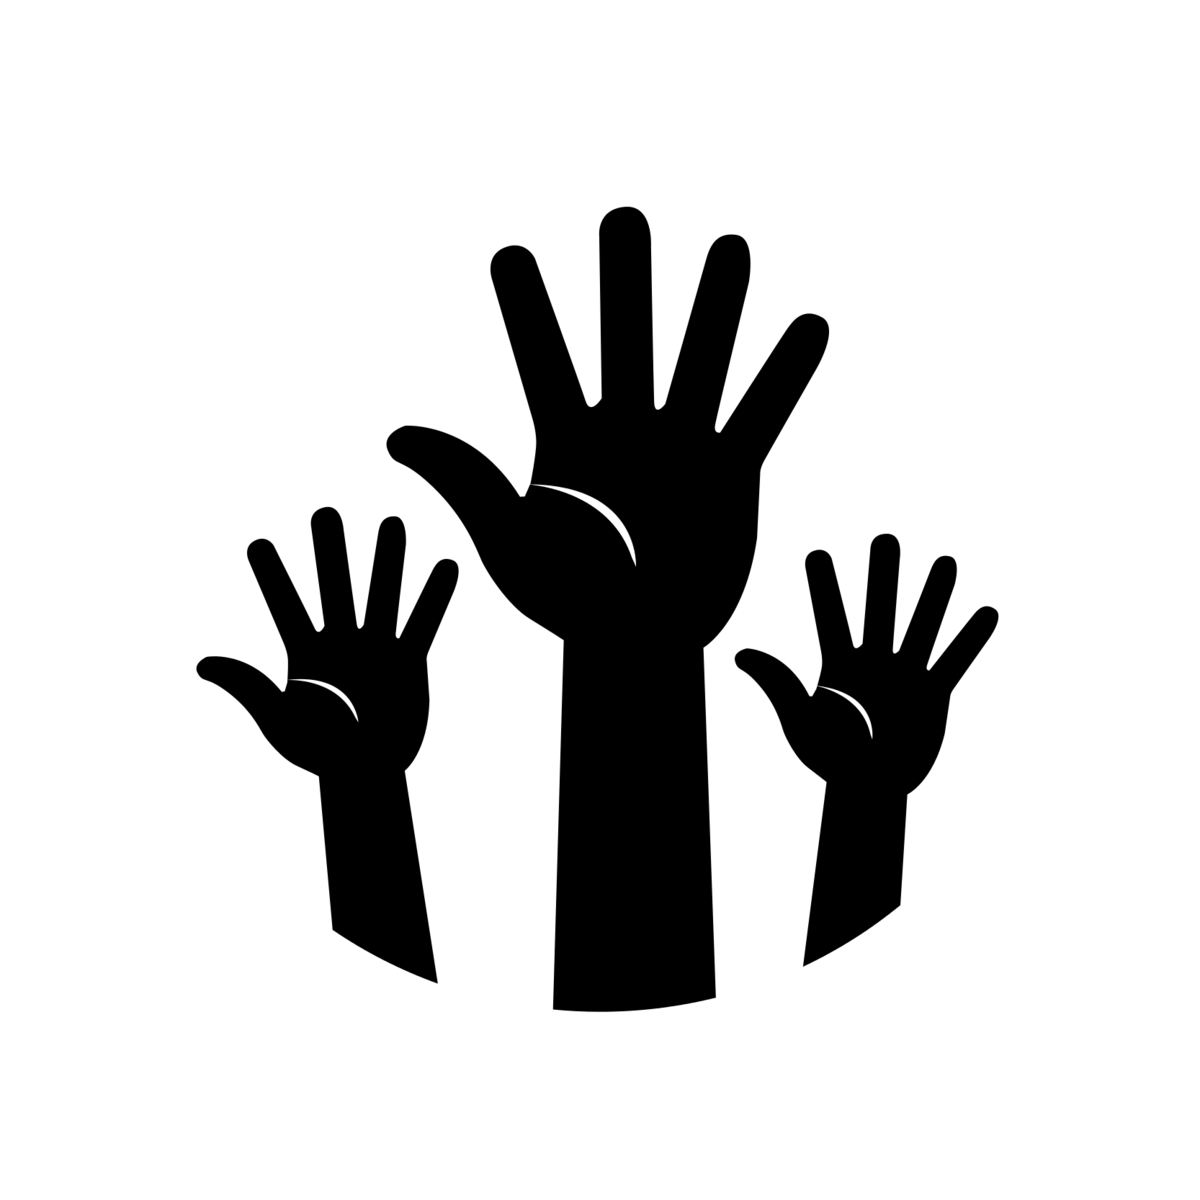
\includegraphics[height=1.5em]{images/hands}}
\newcommand{\transpose}[0]{{\textrm{\tiny{\sf{T}}}}}
\newcommand{\norm}{{\mathcal{N}}}
\newcommand{\cutoff}[0]{\kappa}
\newcommand{\instD}[0]{\dataset}
\newcommand{\insts}[0]{\mathcal{I}}
\newcommand{\inst}[0]{i}
\newcommand{\instI}[1]{i^{(#1)}}

% Iteration specific instance of variable/function/anything
% Introduced in the BO section, but moved up here to make it available within other macros
\newcommand{\iter}[2][\bocount]{{#2}^{(#1)}}

%--------HPO parameter macros-----------

% Parameter Configuration Space
\newcommand{\pcs}[0]{\pmb{\Lambda}}

% ???
\newcommand{\bx}[0]{\conf}

% Parameter Configuration
\newcommand{\conf}[0]{\pmb{\lambda}}

% Final Configuration
\newcommand{\finconf}[0]{\pmb{\hat{\lambda}}}

% Configuration corresponding to a given iteration -- better use \iter!
\newcommand{\confI}[1]{{\conf}^{(#1)}}

% Default Configuration
\newcommand{\defconf}[0]{{\conf}_{\text{def}}}

% Incumbent Configuration
\newcommand{\incumbent}[1][\bocount]{\iter[#1]{\finconf}}

% Optimal Configuration
\newcommand{\optconf}[0]{{\conf}^*}

% Configuration Space
\newcommand{\confs}[0]{\pcs}

%----------------------------------------

%\newcommand{\vlambda}[0]{\bm{\lambda}}
%\newcommand{\vLambda}[0]{\bm{\Lambda}}
\newcommand{\dataset}[0]{\mathcal{D}}
\newcommand{\datasets}[0]{\mathbf{D}}
\newcommand{\loss}[0]{L}
\newcommand{\risk}{\mathcal{R}}
\newcommand{\riske}{\mathcal{R}_{\text{emp}}}
\newcommand{\cost}[0]{c}
\newcommand{\costI}[1]{c^{(#1)}}

% Gaussian Process
\newcommand{\gp}{\mathcal{G}}
% Family of Objective Functions
\newcommand{\objF}{F}

%---------------BO Macros------------------

% BO loop counter
\newcommand{\bocount}{t}
% BO loop counter max, the counter runs from 1 to this value
\newcommand{\bobudget}{T}
% BO loop observation
\newcommand{\obs}[1][\conf]{\cost({#1})}
% BO loop observation space
\newcommand{\obsspace}{\mathcal{Y}}
% BO loop next observation
\newcommand{\bonextobs}{\obs[\iter{\conf}]}
% Acquisition Function, no args
\newcommand{\acq}{u}
% Standard Normal PDF
\newcommand{\pdf}{\phi}
% Standard Normal CDF
\newcommand{\cdf}{\Phi}
% Mean
\newcommand{\mean}{\mu}
% Standard Deviation
\newcommand{\stddev}{\sigma}
% Variance
\newcommand{\variance}{\sigma^2}
% Noise
\newcommand{\noise}{\nu}
% BO loop next selected sample
\newcommand{\bonextsample}{\confI{\bocount}}

% Single hyperparameter
\newcommand{\hyperparam}{\lambda}

% Single hyperparameter within a hyperparameter configuration
\newcommand{\hyperparami}[1][i]{{\hyperparam}_#1}

% Full definition of final configuration
\newcommand{\finconffull}{\incumbent[\bobudget]}

% Dataset
\newcommand{\datasetHPO}{{\dataset}_{HPO}}

% Dataset definition
\newcommand{\datasetHPOdef}{{\langle \bonextsample,\,\bonextobs \rangle}_{\bocount=1}^{\bobudget}}

% Double Display Fraction, forces large displays for everything in numerator and denominator
\newcommand\ddfrac[2]{\frac{\displaystyle #1}{\displaystyle #2}}

% Conditional Probability "Given That" Relation, source:https://tex.stackexchange.com/a/141685/205886
\newcommand\given[1][]{\:#1\vert\:}

% Expectation as a math operator
\DeclareMathOperator*{\E}{\mathbb{E}}

% Citation 
\newcommand{\source}[1]{
    \begin{flushright}
    	Source: \lit{#1}
    \end{flushright}
}
%-------------------------------------------

%Real numbers set
\newcommand{\realnum}{\mathbb{R}}
%Configuration space - do not use
%\newcommand{\configspace}{\Theta}
%Instances - do not use
%\newcommand{\instances}{\mathcal{I}}
%Expected value
\newcommand{\expectation}{\mathbb{E}}
%Kernel
\newcommand{\kernel}{\kappa}
%Constraint function
\newcommand{\constraintf}{c}
%Normal distribution
\newcommand{\normaldist}{\mathcal{N}}

% \renewcommand{\vec}[1]{\mathbf{#1}}
\newcommand{\hist}[0]{\dataset_{\text{Hist}}}
\newcommand{\param}[0]{p}
\newcommand{\algo}[0]{\mathcal{A}}
\newcommand{\algos}[0]{\mathbf{A}}
%\newcommand{\nn}[0]{N}
\newcommand{\feats}[0]{\mathcal{X}_{\text{meta}}}
\newcommand{\feat}[0]{\x_{\text{meta}}}
%\newcommand{\cluster}[0]{\vec{h}}
%\newcommand{\clusters}[0]{\vec{H}}
\newcommand{\perf}[0]{\mathbb{R}}
%\newcommand{\surro}[0]{\mathcal{S}}
\newcommand{\surro}[0]{\hat{\cost}}
\newcommand{\func}[0]{f}
\newcommand{\epm}[0]{\surro}
\newcommand{\portfolio}[0]{\mathbf{P}}
\newcommand{\schedule}[0]{\mathcal{S}}

% Machine Learning
\newcommand{\mdata}[0]{\dataset_{\text{meta}}}
\newcommand{\datasettrain}[0]{\dataset_{\text{train}}}
\newcommand{\datasetval}[0]{\dataset_{\text{val}}}
\newcommand{\datasettest}[0]{\dataset_{\text{test}}}
\newcommand{\x}[0]{\mathbf{x}}
\newcommand{\y}[0]{y}
\newcommand{\xI}[1]{\mathbf{x}^{(#1)}}
\newcommand{\yI}[1]{y^{(#1)}}
\newcommand{\fx}{f(\mathbf{x})}  % f(x), continuous prediction function
\newcommand{\Hspace}{\mathcal{H}} % hypothesis space where f is from
\newcommand{\fh}{\hat{f}}       % f hat, estimated prediction function

% Deep Learning
\newcommand{\weights}[0]{\theta}
\newcommand{\metaweights}[0]{\phi}


% reinforcement learning
\newcommand{\policies}[0]{\mathbf{\Pi}}
\newcommand{\policy}[0]{\pi}
\newcommand{\actionRL}[0]{a}
\newcommand{\stateRL}[0]{s}
\newcommand{\statesRL}[0]{\mathcal{S}}
\newcommand{\rewardRL}[0]{r}
\newcommand{\rewardfuncRL}[0]{\mathcal{R}}

\RestyleAlgo{algoruled}
\DontPrintSemicolon
\LinesNumbered
\SetAlgoVlined
\SetFuncSty{textsc}

\SetKwInOut{Input}{Input}
\SetKwInOut{Output}{Output}
\SetKw{Return}{return}

%\newcommand{\changed}[1]{{\color{red}#1}}

%\newcommand{\citeN}[1]{\citeauthor{#1}~(\citeyear{#1})}

\renewcommand{\vec}[1]{\mathbf{#1}}
\DeclareMathOperator*{\argmin}{arg\,min}
\DeclareMathOperator*{\argmax}{arg\,max}

%\newcommand{\aqme}{\textit{AQME}}
%\newcommand{\aslib}{\textit{ASlib}}
%\newcommand{\llama}{\textit{LLAMA}}
%\newcommand{\satzilla}{\textit{SATzilla}}
%\newcommand{\satzillaY}[1]{\textit{SATzilla'{#1}}}
%\newcommand{\snnap}{\textit{SNNAP}}
%\newcommand{\claspfolioTwo}{\textit{claspfolio~2}}
%\newcommand{\flexfolio}{\textit{FlexFolio}}
%\newcommand{\claspfolioOne}{\textit{claspfolio~1}}
%\newcommand{\isac}{\textit{ISAC}}
%\newcommand{\eisac}{\textit{EISAC}}
%\newcommand{\sss}{\textit{3S}}
%\newcommand{\sunny}{\textit{Sunny}}
%\newcommand{\ssspar}{\textit{3Spar}}
%\newcommand{\cshc}{\textit{CSHC}}
%\newcommand{\cshcpar}{\textit{CSHCpar}}
%\newcommand{\measp}{\textit{ME-ASP}}
%\newcommand{\aspeed}{\textit{aspeed}}
%\newcommand{\autofolio}{\textit{AutoFolio}}
%\newcommand{\cedalion}{\textit{Cedalion}}
\newcommand{\fanova}{\textit{fANOVA}}
\newcommand{\sbs}{\textit{SB}}
\newcommand{\oracle}{\textit{VBS}}

% like approaches
\newcommand{\claspfoliolike}[1]{\texttt{claspfolio-#1-like}}
\newcommand{\satzillalike}[1]{\texttt{SATzilla'#1-like}}
\newcommand{\isaclike}{\texttt{ISAC-like}}
\newcommand{\ssslike}{\texttt{3S-like}}
\newcommand{\measplike}{\texttt{ME-ASP-like}}

\newcommand{\irace}{\textit{I/F-race}}
\newcommand{\gga}{\textit{GGA}}
\newcommand{\smac}{\textit{SMAC}}
\newcommand{\paramils}{\textit{ParamILS}}
\newcommand{\spearmint}{\textit{Spearmint}}
\newcommand{\tpe}{\textit{TPE}}


\usepackage{pifont}
\newcommand{\itarrow}{\mbox{\Pisymbol{pzd}{229}}}
\newcommand{\ithook}{\mbox{\Pisymbol{pzd}{52}}}
\newcommand{\itcross}{\mbox{\Pisymbol{pzd}{56}}}
\newcommand{\ithand}{\mbox{\raisebox{-1pt}{\Pisymbol{pzd}{43}}}}

%\DeclareMathOperator*{\argmax}{arg\,max}

\newcommand{\ie}{{\it{}i.e.\/}}
\newcommand{\eg}{{\it{}e.g.\/}}
\newcommand{\cf}{{\it{}cf.\/}}
\newcommand{\wrt}{\mbox{w.r.t.}}
\newcommand{\vs}{{\it{}vs\/}}
\newcommand{\vsp}{{\it{}vs\/}}
\newcommand{\etc}{{\copyedit{etc.}}}
\newcommand{\etal}{{\it{}et al.\/}}

\newcommand{\pscProc}{{\bf procedure}}
\newcommand{\pscBegin}{{\bf begin}}
\newcommand{\pscEnd}{{\bf end}}
\newcommand{\pscEndIf}{{\bf endif}}
\newcommand{\pscFor}{{\bf for}}
\newcommand{\pscEach}{{\bf each}}
\newcommand{\pscThen}{{\bf then}}
\newcommand{\pscElse}{{\bf else}}
\newcommand{\pscWhile}{{\bf while}}
\newcommand{\pscIf}{{\bf if}}
\newcommand{\pscRepeat}{{\bf repeat}}
\newcommand{\pscUntil}{{\bf until}}
\newcommand{\pscWithProb}{{\bf with probability}}
\newcommand{\pscOtherwise}{{\bf otherwise}}
\newcommand{\pscDo}{{\bf do}}
\newcommand{\pscTo}{{\bf to}}
\newcommand{\pscOr}{{\bf or}}
\newcommand{\pscAnd}{{\bf and}}
\newcommand{\pscNot}{{\bf not}}
\newcommand{\pscFalse}{{\bf false}}
\newcommand{\pscEachElOf}{{\bf each element of}}
\newcommand{\pscReturn}{{\bf return}}

%\newcommand{\param}[1]{{\sl{}#1}}
\newcommand{\var}[1]{{\it{}#1}}
\newcommand{\cond}[1]{{\sf{}#1}}
%\newcommand{\state}[1]{{\sf{}#1}}
%\newcommand{\func}[1]{{\sl{}#1}}
\newcommand{\set}[1]{{\Bbb #1}}
%\newcommand{\inst}[1]{{\tt{}#1}}
\newcommand{\myurl}[1]{{\small\sf #1}}

\newcommand{\Nats}{{\Bbb N}}
\newcommand{\Reals}{{\Bbb R}}
\newcommand{\extset}[2]{\{#1 \; | \; #2\}}

\newcommand{\vbar}{$\,\;|$\hspace*{-1em}\raisebox{-0.3mm}{$\,\;\;|$}}
\newcommand{\vendbar}{\raisebox{+0.4mm}{$\,\;|$}}
\newcommand{\vend}{$\,\:\lfloor$}


\newcommand{\goleft}[2][.7]{\parbox[t]{#1\linewidth}{\strut\raggedright #2\strut}}
\newcommand{\rightimage}[2][.3]{\mbox{}\hfill\raisebox{1em-\height}[0pt][0pt]{\includegraphics[width=#1\linewidth]{#2}}\vspace*{-\baselineskip}}





%\newcommand{\a}[0]{\mathbf{a}}
%\newcommand{\y}[0]{\mathbf{y}}
\newcommand{\q}[0]{\mathbf{q}}
\newcommand{\Xspace}[0]{\mathcal{X}}

\title[AutoML: Overview]{Multi-criteria Optimization}
\subtitle{Bayesian Optimization}
%TODO: change authors!
\author[Bernd Bischl]{\underline{Bernd Bischl} \and Frank Hutter \and Lars Kotthoff\newline \and Marius Lindauer \and Joaquin Vanschoren}
\institute{}
\date{}



% \AtBeginSection[] % Do nothing for \section*
% {
%   \begin{frame}{Outline}
%     \bigskip
%     \vfill
%     \tableofcontents[currentsection]
%   \end{frame}
% }

\begin{document}

	\maketitle



\begin{frame}[allowframebreaks]{Recap: Bayesian Optimization}

Remember the advantages of Bayesian optimization:

\begin{block}{Advantages}
\begin{itemize}
  \item Sample efficient
  \item Can handle noise
  \item Native incorporation of priors
  \item Does not require gradients
  \item Theoretical guarantees
\end{itemize}
\end{block}

To achieve all these advantages for multi-criteria problems, we want to extend Bayesian optimization to multiple cost functions.

\framebreak

\begin{center}
\begin{minipage}{0.75\textwidth}
\begin{algorithm}[H]
    %\DontPrintSemicolon
%    \SetAlgoLined
    \setcounter{AlgoLine}{0}
    \SetKwInOut{Require}{Require}
    \SetKwInOut{Result}{Result}

    \Require{Search space $\pcs$,
    		cost function $\cost$,
    		acquisition function $\acq$, predictive model $\surro$,
    		maximal number of function evaluations $\bobudget$}
    \Result{Best configuration $\finconf$
    (according to $\dataset$ or
    $\surro$)}

	Initialize data $\iter[0]{\dataset}$ with initial observations\;% \leftarrow \varnothing$\;

    \For{$\bocount=1$ \KwTo $\bobudget$}{
		%\While{$B$ not exhausted} {
		Fit predictive model $\iter[\bocount]{\surro}$ on $\iter[\bocount-1]{\dataset}$\;

		Select next query point: $\bonextsample \in \argmax_{\conf \in \pcs} \acq(\conf; \iter[\bocount-1]{\dataset}, \iter[\bocount]{\surro})$\;

		Query $\bonextobs$\;

		Update data: $\iter[\bocount]{\dataset} \leftarrow \iter[\bocount-1]{\dataset} \cup \{\langle \bonextsample, \bonextobs \rangle \}$\;
	}
	\caption*{Bayesian optimization loop}
\end{algorithm}
\end{minipage}
\end{center}
\end{frame}


\begin{frame}{Multi-Criteria Bayesian Optimization}

\textbf{Goal}: Extend Bayesian optimization to multiple cost functions

$$
\min_{\conf \in \pcs}  \cost(\conf) \Leftrightarrow \min_{\conf \in \pcs} \left(\cost_1(\conf), \cost_2(\conf), ..., \cost_m(\conf)\right).
$$


    \vspace{0.5cm}

There are two basic approaches:

\begin{enumerate}
        \item Simplify the problem by scalarizing the cost functions, or
        \item define acquisition functions for multiple cost functions.
\end{enumerate}

\end{frame}

\begin{frame}{Scalarization}

    \textbf{Idea:} Aggregate all cost functions


    $$\min_{\conf \in \pcs} \sum_{i = 1}^m w_i \cost_i(\conf) \qquad \text{with} \quad w_i \ge 0 $$

    \begin{itemize}
        \item \textbf{Obvious problem:} How to choose $w_1, \dots, w_m$?
            \begin{itemize}
                \item Expert knowledge?
                \item Systematic variation?
                \item Random variation?
            \end{itemize}
        \item If expert knowledge is not available a-priori, we need to ensured that different trade-offs between the cost functions are explored.
            \item Simplifies multi-criteria optimization problem to single-objective \\$\longrightarrow$ Bayesian optimization can be used without adaptions of the general algorithm.
    \end{itemize}

\end{frame}

\begin{frame}{Scalarization: ParEGO~\litw{\href{https://doi.org/10.1109/TEVC.2005.851274}{Knowles et al. 2006}}}

    Scalarize the cost functions using the augmented Tchebycheff norm

    $$
    c = \max_{i=1,\dots,m}\left(w_i \cost_i(\conf)\right) + \rho \sum_{i=1}^m w_i\cost_i(\conf),
    $$

    \begin{itemize}
        \item The weights $w \in W$ are drawn from
            $$
                W = \left\{ w = (w_1, \dots, w_m) | \sum_{i=1}^m w_i = 1, w_i = \frac{l}{s} \wedge, l \in 0,\dots,s\right\},
            $$
            with $|W| = {{s+m-1}\choose{k-1}}1$.
        \item New weights are drawn in every BO iteration.
        \item $\rho$ is a small parameter suggested to be set to $0.05$.
        \item $s$ selects the number of different weights to draw from.
    \end{itemize}

\end{frame}

\begin{frame}{Why the Tchebycheff norm?}

    \begin{center}
        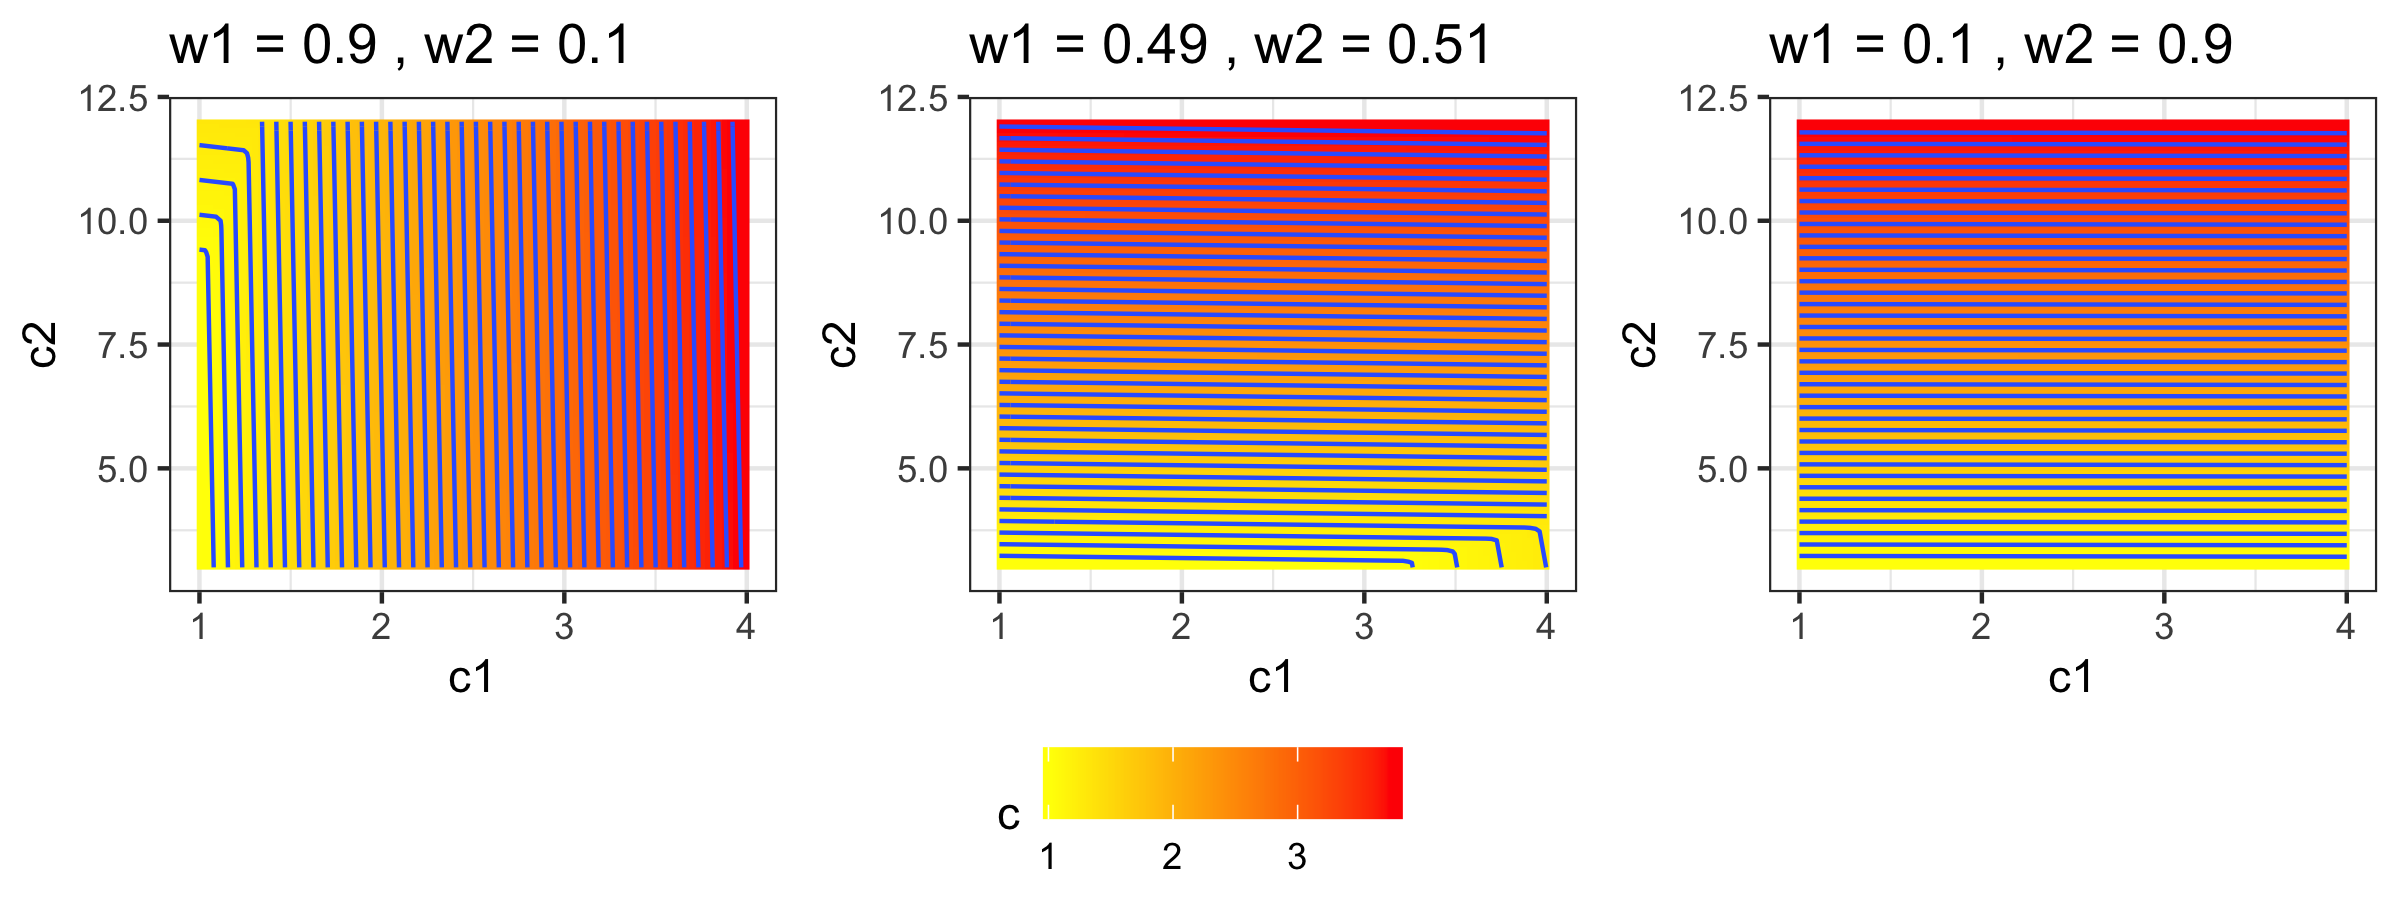
\includegraphics[scale=0.1]{images/parego_viz}
    \end{center}
        %Example of 3 different ParEGO scalarizations of the two objective functions $\cost_1(\conf) = (\conf - 1)^2$ and $c_2(\conf) = 3(\conf - 2)^2$.
    $$
    c = \max_{i=1,\dots,m}\left(w_i \cost_i(\conf)\right) + \rho \sum_{i=1}^m w_i\cost_i(\conf),
    $$
    \begin{scriptsize}
    \begin{itemize}
        \item The norm consists of two components:
            \begin{itemize}
                    \item $\max_{i=1,\dots,m}\left(w_i \cost_i(\conf)\right)$ takes only the cost function with maximum weight into account.
                    \item $\sum_{i=1}^m w_i\cost_i(\conf)$ is the weighted sum of all cost functions.
            \end{itemize}
        \item $\rho$ describes the trade-off between these components.
        \item By the randomized weights in each iteration and the usually small value of $\rho = 0.05$, this allows exploration of extreme points of single cost functions.
    \end{itemize}
    \end{scriptsize}
\end{frame}

\begin{frame}{ParEGO Algorithm}


\begin{center}
\begin{minipage}{0.8\textwidth}
\begin{algorithm}[H]
    %\DontPrintSemicolon
%    \SetAlgoLined
    \setcounter{AlgoLine}{0}
    \SetKwInOut{Require}{Require}
    \SetKwInOut{Result}{Result}

    \Require{Search space $\pcs$,
    		cost function $\cost$,
    		acquisition function $\acq$, predictive model $\surro$,
            maximal number of function evaluations $\bobudget$, $\rho$, $l$, $s$}
    \Result{Best configuration $\finconf$
    (according to $\dataset$ or
    $\surro$)}

	Initialize data $\iter[0]{\dataset}$ with initial observations\;% \leftarrow \varnothing$\;

    \For{$\bocount=1$ \KwTo $\bobudget$}{
		%\While{$B$ not exhausted} {
        Sample $w$ from  $\left\{ w = (w_1, \dots, w_m) | \sum_{i=1}^m w_i = 1, w_i = \frac{l}{s} \wedge, l \in 0,\dots,s\right\}$;

        Compute scalarization $c^{(t)} = \max_{i=1,\dots,m}\left(w_i \cost_i(\conf)\right) + \rho \sum_{i=1}^m w_i\cost_i(\conf)$;

		Fit predictive model $\iter[\bocount]{\surro}$ on $\iter[\bocount-1]{\dataset}$\;

		Select next query point: $\bonextsample \in \argmax_{\conf \in \pcs} \acq(\conf; \iter[\bocount-1]{\dataset}, \iter[\bocount]{\surro})$\;

		Query $\bonextobs$\;

		Update data: $\iter[\bocount]{\dataset} \leftarrow \iter[\bocount-1]{\dataset} \cup \{\langle \bonextsample, \bonextobs \rangle \}$\;
	}
	\caption*{ParEGO loop}
\end{algorithm}
\end{minipage}
\end{center}
\end{frame}


%\begin{frame}{ParEGO Example}

%    \begin{center}
%        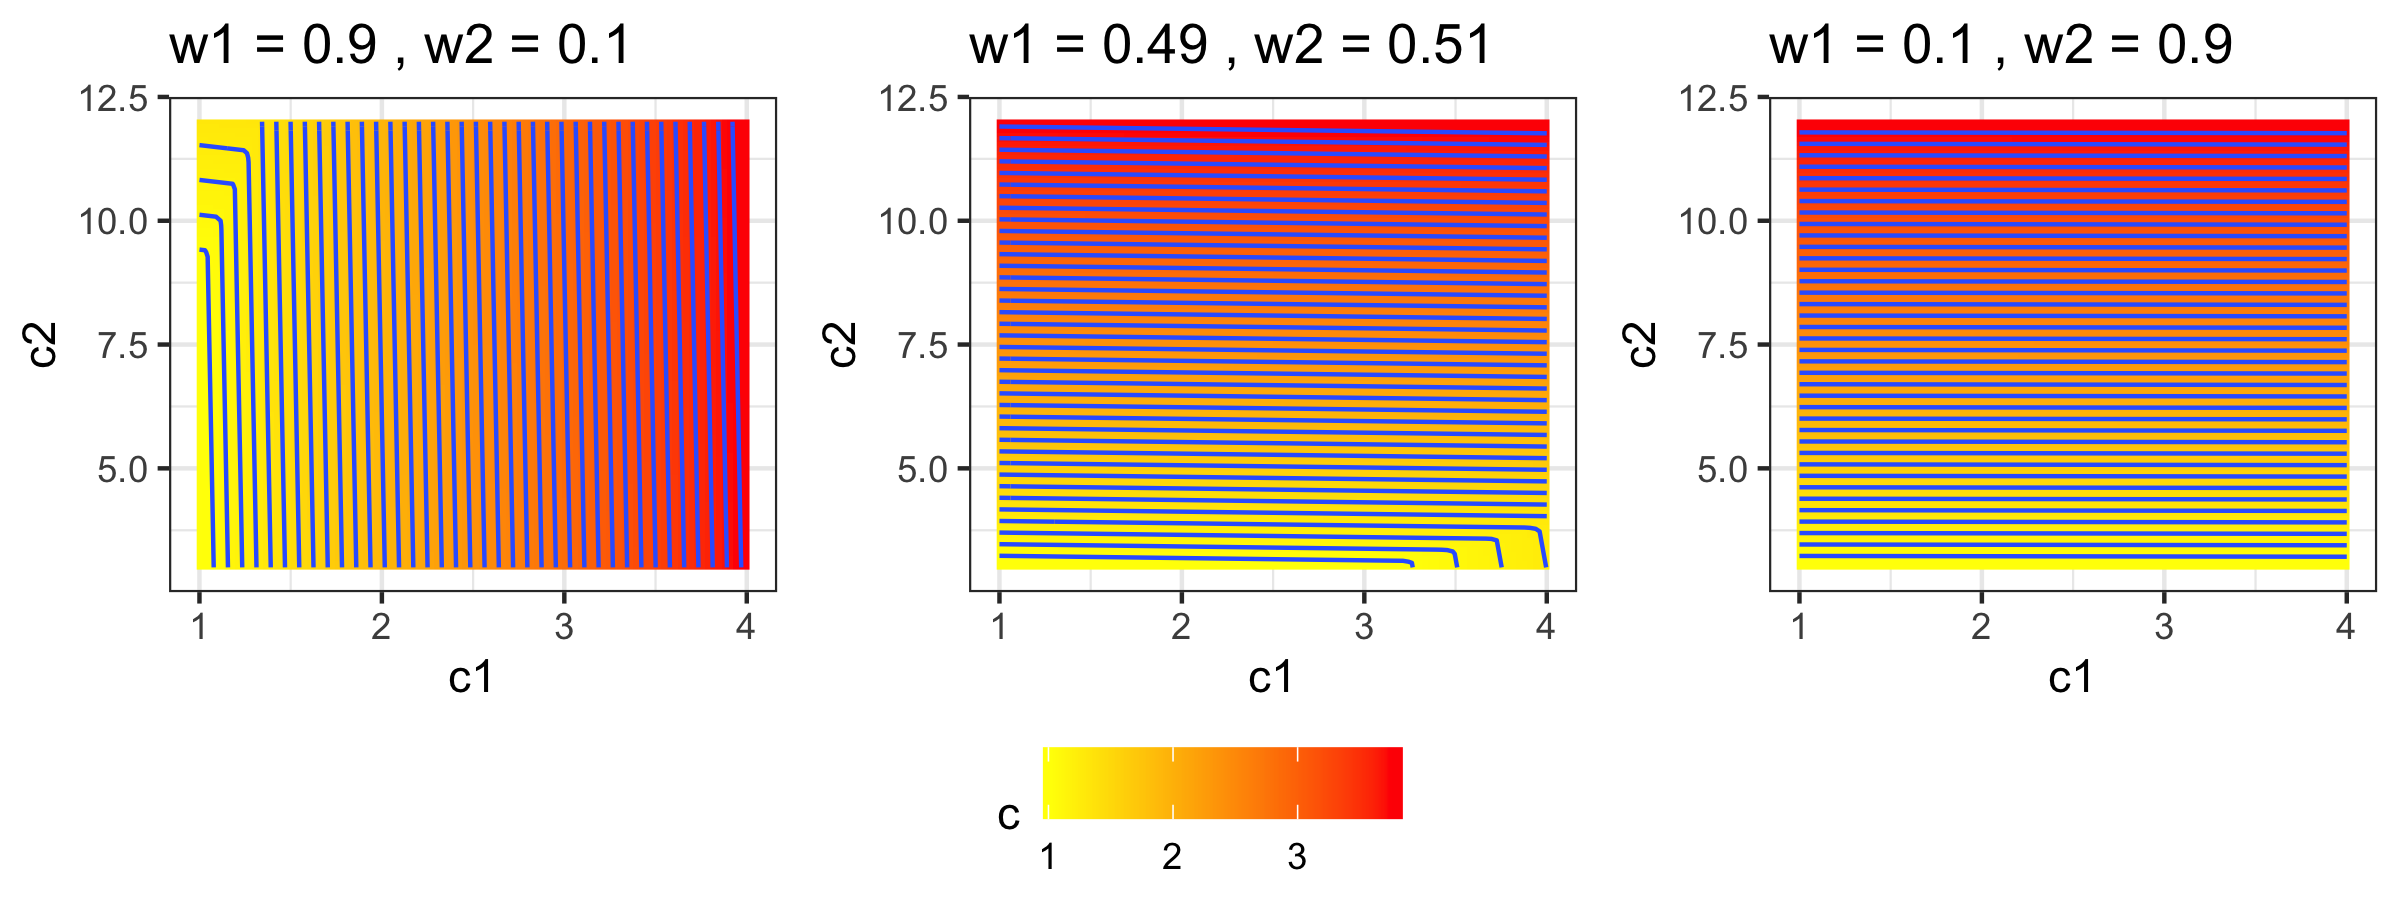
\includegraphics[scale=0.15]{images/parego_viz}
%    \end{center}
%        Example of 3 different ParEGO scalarizations of the two objective functions $\cost_1(\conf) = (\conf - 1)^2$ and $c_2(\conf) = 3(\conf - 2)^2$.
%\end{frame}


\begin{frame}{Hypervolume based Acquisition Functions}

    \textbf{Idea:} Define acquisition function that directly models contribution to the dominated hypervolume.

            $$
            \max(0, S(\mathcal{P} \cup \conf, R) - S(\mathcal{P}, R))
            $$
    \begin{center}
        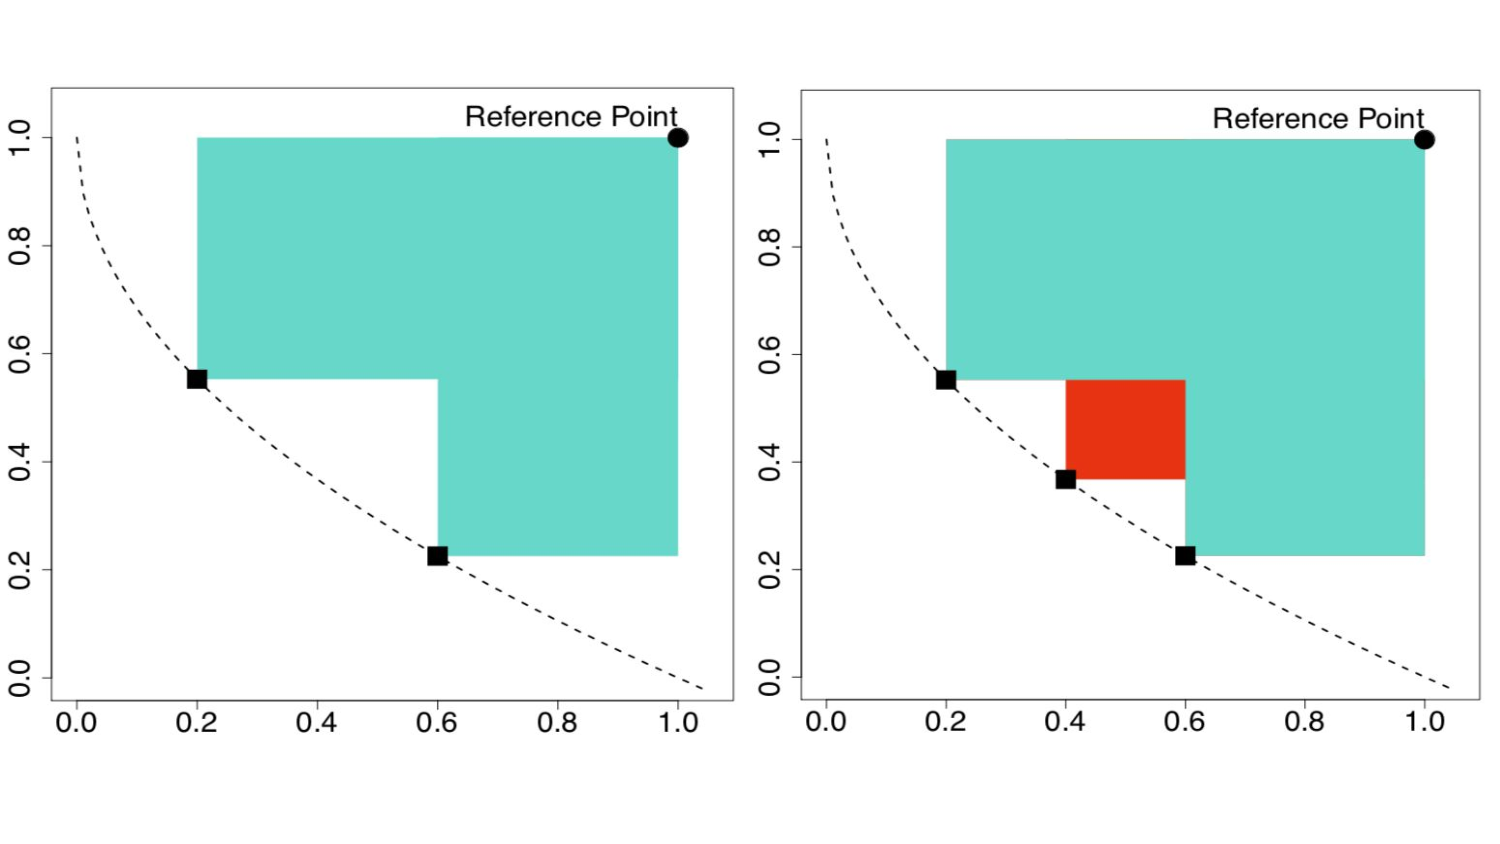
\includegraphics[scale=0.22]{images/hv_contribution}
    \end{center}

    \begin{itemize}
            \item Fit $m$ single-objective surrogate models $\surro_1, \dots, \surro_m$
            \item Acquisition function takes all surrogate models into account.
            \item Single-criteria optimization of acquisition function.
    \end{itemize}

\end{frame}

\begin{frame}[allowframebreaks]{S-Metric Selection-based EGO}

    Using the Lower Confidence bound $u_{\text{LCB}, 1}(\conf), \dots, u_{\text{LCB}, m}(\conf)$, an optimistic estimate of hypervolume contribution can be calculated.

    \begin{center}
        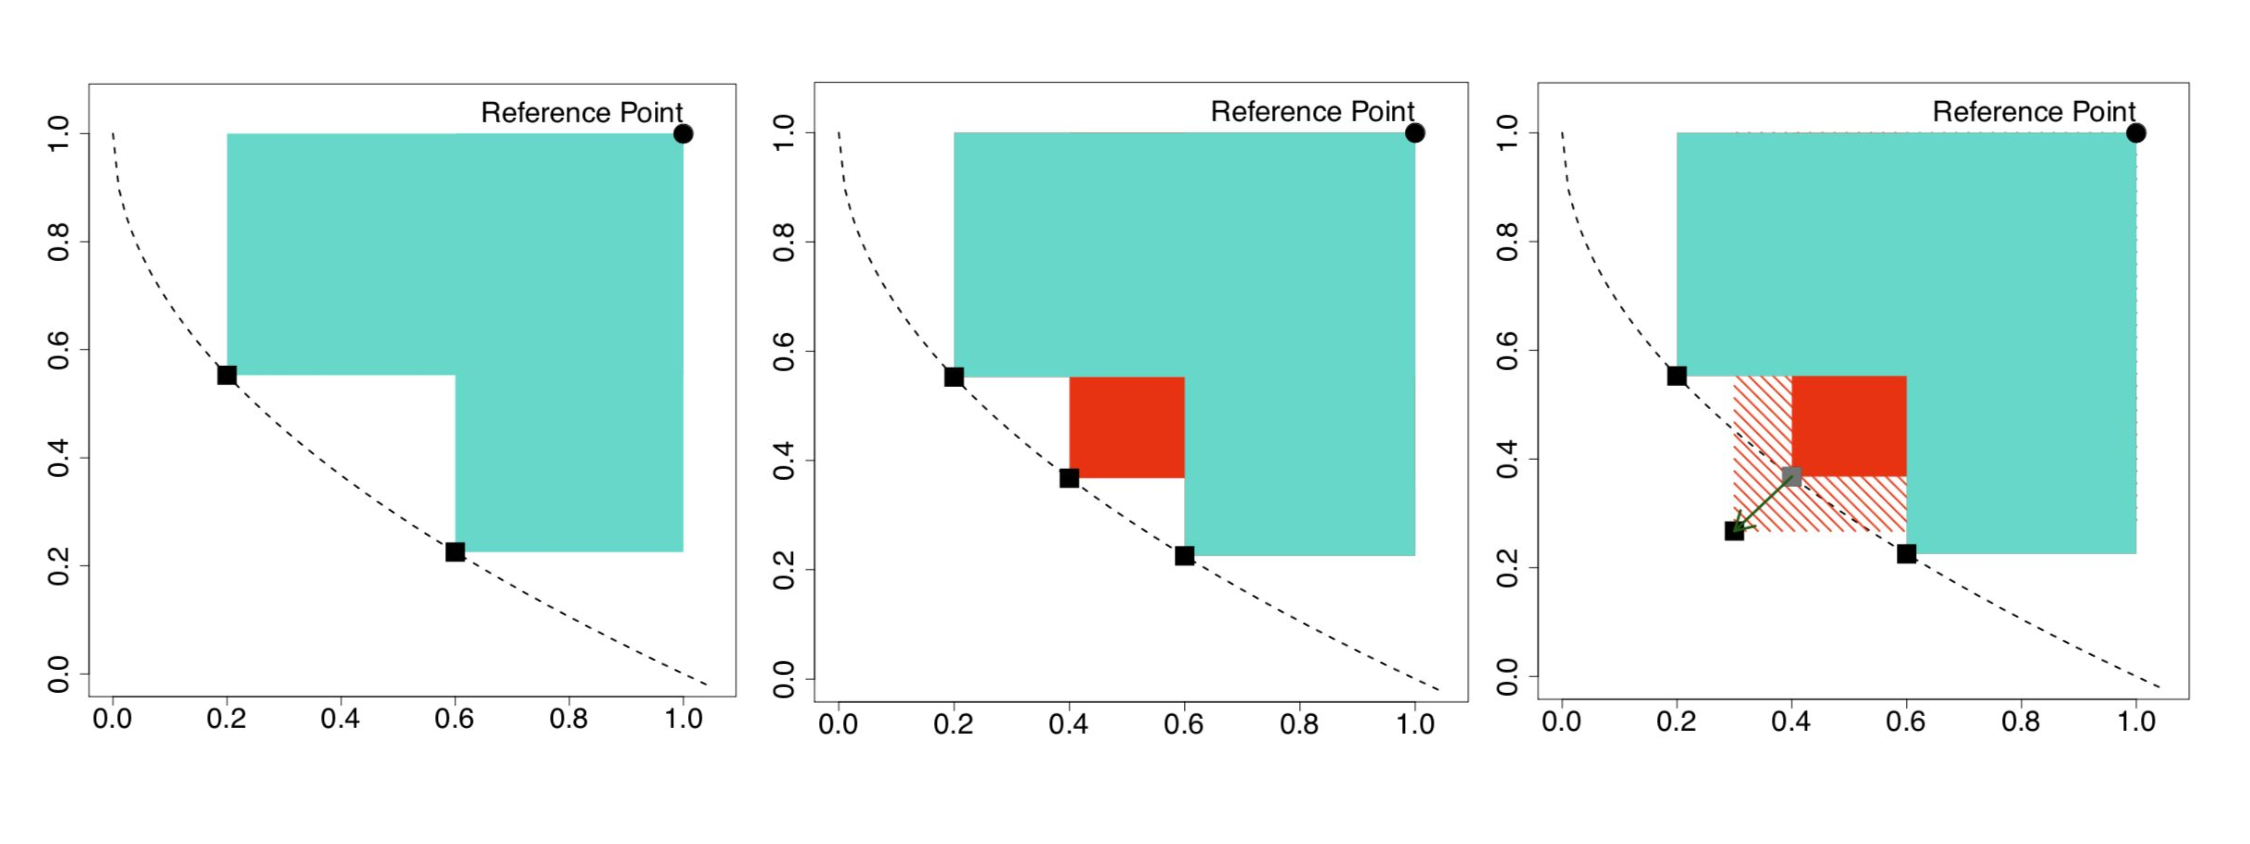
\includegraphics[scale=0.35]{images/hv_contribution_2}
    \end{center}

    \framebreak

    As potential solution can be predicted beyond the real objective space, additive $\epsilon$-dominance ($\preceq_\epsilon$) is measured
            $$
                c_1(\conf^{(i)}) \le \epsilon+c_1(\conf^{(j)}), \dots, c_m(\conf^{(i)}) \le \epsilon+c_m(\conf^{(j)}),
            $$
            and a penalty is applied to these configurations
            $$
                \Psi(\conf) = -1 + \prod_{j=1}^m(1+u(\conf)_j - c_j).
            $$

    \begin{itemize}
        \item This method is referred to as SMS-EGO~\litw{\href{https://doi.org/10.1007/978-3-540-87700-4_78}{Ponweiser et al. 2008}}.
    \end{itemize}
\end{frame}

\begin{frame}{Further Hypervolume based Acquisition Functions}

    \textbf{Expected Hypervolume Improvement (EHI)}~\litw{\href{https://doi.org/10.1016/j.swevo.2018.10.007}{Yang et al. 2019}}

$$
    u_{EI, \mathcal{H}}(\conf) = \int_{-\infty}^{\infty} p(\cost \mid \conf) \times \mathcal{H}(\conf)\;\; d\cost,\
$$
    with $\mathcal{H}(\conf) = S(\mathcal{P} \cup \conf, R) - S(\mathcal{P}, R))$.

    \begin{itemize}
        \item Direct extension of $u_{EI}$ to the hypervolume.
        \item $p(\cost \mid \conf)$ is the joint density of the surrogate model predictions at $\conf$.
        \item As the surrogates are GPs and modeled independently of each other, this is just an integral over $m$ univariate normal distributions.
        \item Efficient computations for $m \le 3$ exist, beyond that expensive simulation-based computation is required.
    \end{itemize}


    \vspace{0.5cm}
Further hypervolume based acquisition functions:

    \begin{itemize}
        \item \textbf{Stepwise Uncertainty Reduction} (SUR) based on the probability of improvement.
        \item \textbf{Expected Maximin Improvement} (EMI) based on the $\epsilon$-indicator.
    \end{itemize}


\end{frame}

\begin{frame}{Hypervolume based BO Algorithm}


\begin{center}
\begin{minipage}{0.8\textwidth}
\begin{algorithm}[H]
    %\DontPrintSemicolon
%    \SetAlgoLined
    \setcounter{AlgoLine}{0}
    \SetKwInOut{Require}{Require}
    \SetKwInOut{Result}{Result}

    \Require{Search space $\pcs$,
    		cost function $\cost$,
    		acquisition function $\acq$, predictive model $\surro$,
            maximal number of function evaluations $\bobudget$}
    \Result{Best configuration $\finconf$
    (according to $\dataset$ or
    $\surro$)}

	Initialize data $\iter[0]{\dataset}$ with initial observations\;% \leftarrow \varnothing$\;

    \For{$\bocount=1$ \KwTo $\bobudget$}{
		%\While{$B$ not exhausted} {

		Fit predictive models $\iter[\bocount]{\surro_1}, \dots, \iter[\bocount]{\surro_m}$ on $\iter[\bocount-1]{\dataset}$\;

		Select next query point: $\bonextsample \in \argmax_{\conf \in \pcs} \acq(\conf; \iter[\bocount-1]{\dataset}, \iter[\bocount]{\surro_1}, \dots, \iter[\bocount]{\surro_m}))$\;

		Query $\bonextobs$\;

		Update data: $\iter[\bocount]{\dataset} \leftarrow \iter[\bocount-1]{\dataset} \cup \{\langle \bonextsample, \bonextobs \rangle \}$\;
	}
	\caption*{Hypervolume based Bayesian optimization loop}
\end{algorithm}
\end{minipage}
\end{center}
\end{frame}

% NOTE: We decided to scrap mspot
% \begin{frame}{Multi-Criteria Optimization of Acquisition Functions}
%     \textbf{Goal:} Apply multi-criteria optimization methods on acquisition to approximate a pareto front.

%     \begin{itemize}
%        \item Separate surrogate model $\surro_1, \dots, \surro_m$ for each cost function.
%        \item Apply Multi-Criteria optimization (e.g. NSGA-II) to approximate pareto front over acquisition functions.
%        \item Select a single configuration from the estimated pareto front, e.g., by hypervolume contribution.
%     \end{itemize}
% \end{frame}


\end{document}
